
\section{Experiment}
We design and perform several experiments to evaluate our framework and prove that CLIC is capable of 1) selecting a suitable platform based on the workload and 2) building and running workflows on multiple platforms that are not supported by existing frameworks. 

\subsection{Experimental Setup}
All experiments are conducted on a cluster of 3 nodes, where each node is equipped with two 2.3 GHz Intel Xeon Gold 5218 processors with 16 cores, four 32GB DDR4 RAM, 2TB SSD and runs on 64-bit Ubuntu 20.0.1. The platforms deployed on the cluster include Java’s Stream library (JavaStream), Spark 2.4.5 (Spark), Spark ML 2.4.5 (Spark ML), GraphX 2.4.5 (GraphX), JgraphT 1.4.0 (JgraphT), GraphChi 0.2.2 (GraphChi), Giraph 1.3.9 (Giraph), PyTorch 1.7.1 (PyTorch), python gensim library (gensim). The platform images and containers are managed by Kubernetes v1.20. Alluxio 2.4 is used for data orchestration and HDFS 3.2.1 works as the backend file system.


\subsection{Performance Evaluation of A Single Operator}
\begin{figure}
  \centering
  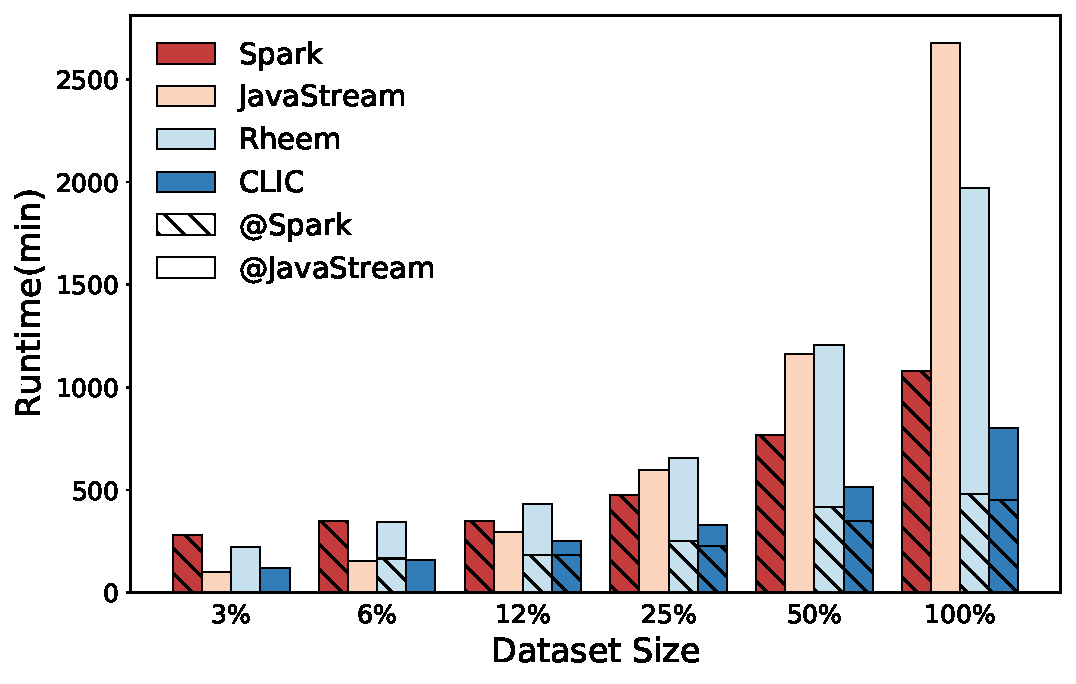
\includegraphics[width=0.7\linewidth]{figures/chp6-CrimeStage.pdf}
  \caption{Performance of London crime analysis}
  \label{fig:exp-crime}
\end{figure}

Figure \ref{fig:single-opt-selection} shows the performance of four representative operators i.e., Word2Vec, PCA, PageRank, and WordCount. In the figures, the platform chosen by the GCN model in CLIC is indicated by red stars. In the evaluation of Word2Vec (Figure \ref{fig:single-word2vec}), we use the NLTK dataset containing the different sizes of corpora to represent different workloads. Among supported platforms, gensim achieves the highest performance when using the corpus of 10k vocabularies while Spark ML suffers from the distributed communication overheads. However, Spark ML gains a performance advantage when the corpus contains 270k vocabularies. This is because Spark ML is able to utilize multiple nodes for the enlarged dataset, where the communication overheads become subtle compared with the computing time. CLIC identifies the difference and selects the best platform in both situations. Figure \ref{fig:single-PCA} shows the accumulated time of 10 PCA runs. The dataset is the Hotel Booking Demand \footnote{https://www.kaggle.com/jessemostipak/hotel-booking-demand}. Consider that running PCA in a single time has negligible performance difference on PyTorch, scikit-learn and Tensorflow for all dataset sizes, we set the feature vectors of these physical operators as the same to reduce the data amount required by training the GCN. Therefore, CLIC selects PyTorch all the time. The data set in evaluating PageRank is the Twitter follower network\footnote{https://snap.stanford.edu/data/twitter-2010.html}. As shown in Figure \ref{fig:single-PR}, JgraphT achieves the highest performance when the graph contains less than 1.8 million vertexes while Giraph performs the best on the other cases for its higher efficiency in processing large graphs. To evaluate the map-reduce operators, we encapsulate the WordCount as a coarse-grained operator. As shown in Figure \ref{fig:single-wc}, the single-machine framework JavaStream achieves the highest when the corpus is small. Instead, Spark is 4.2X faster than JavaStream when using the full dataset because it can be divided and computed locally on each node with little global synchronizing overheads. CLIC selects the best platform for both the PageRank and WordCount operators.

The above experiments validate that CLIC is capable of enhancing the performance of an operator by selecting its appropriate platform.

\subsection{Performance Evaluation of A Big Data Workflow}

Figure \ref{fig:exp-crime} compares the performance of a workflow that analyzes the London Crime dataset\footnote{https://www.kaggle.com/LondonDataStore/london-crime}, which size is 28 GB. The dataset describes the amounts of criminal reports by month, major/minor category, etc. We use percentages in the figure to denote different sizes of the dataset. For instance, 50\% means the execution time on only 14 GB of data (28$\times$0.5).

The workflow mainly consists of the following four procedures: 1) reading data and transforming it to a computable format; 2) filtering reports to preserve only the ones with certain crime types, which will remove 90\% of the data; 3) sorting and transforming reports to a human-readable format, and 4) grouping reports based on quarter. We evaluate the performance on JavaStream and Spark, as well as cross-platform frameworks Rheem and CLIC. 

The observation is that when the data size is less than 6\%, the computational efficiency of native Java and CLIC is 2.1$\times$ higher than Rheem and 2.8$\times$ higher than Spark. The reason is that Spark is always set to use all available nodes in a cluster even when the dataset is small. Consequently, the communication overheads among distributed workers dominate the execution time. Both CLIC and Rheem select the JavaStream for all operators in a small dataset except that JavaStream operators in Rheem are implemented with a single thread which leads to lower performance than the multi-threaded implementations in CLIC. When the dataset size is larger than 12\%, the amount of data to be processed in the first two procedures is too large that moving 
the computation from JavaStream to Spark can benefit from the distributed computing. This is the reason that CLIC starts to outperform the native JavaStream. This benefit is most obvious when the dataset size reaches 100\% where native JavaStream's efficiency is 2.4$\times$ lower than Spark and 3.3$\times$ lower than CLIC. %Although Rheem and CLIC make the same choice, Rheem’s single thread operators are still the bottleneck while CLIC achieves higher performance through  platform selection.


\subsection{Performance Evaluation for Workflows with Multiple Algebras}

\begin{figure}
  \centering
  \subfigure[Sentiment Classification]{
  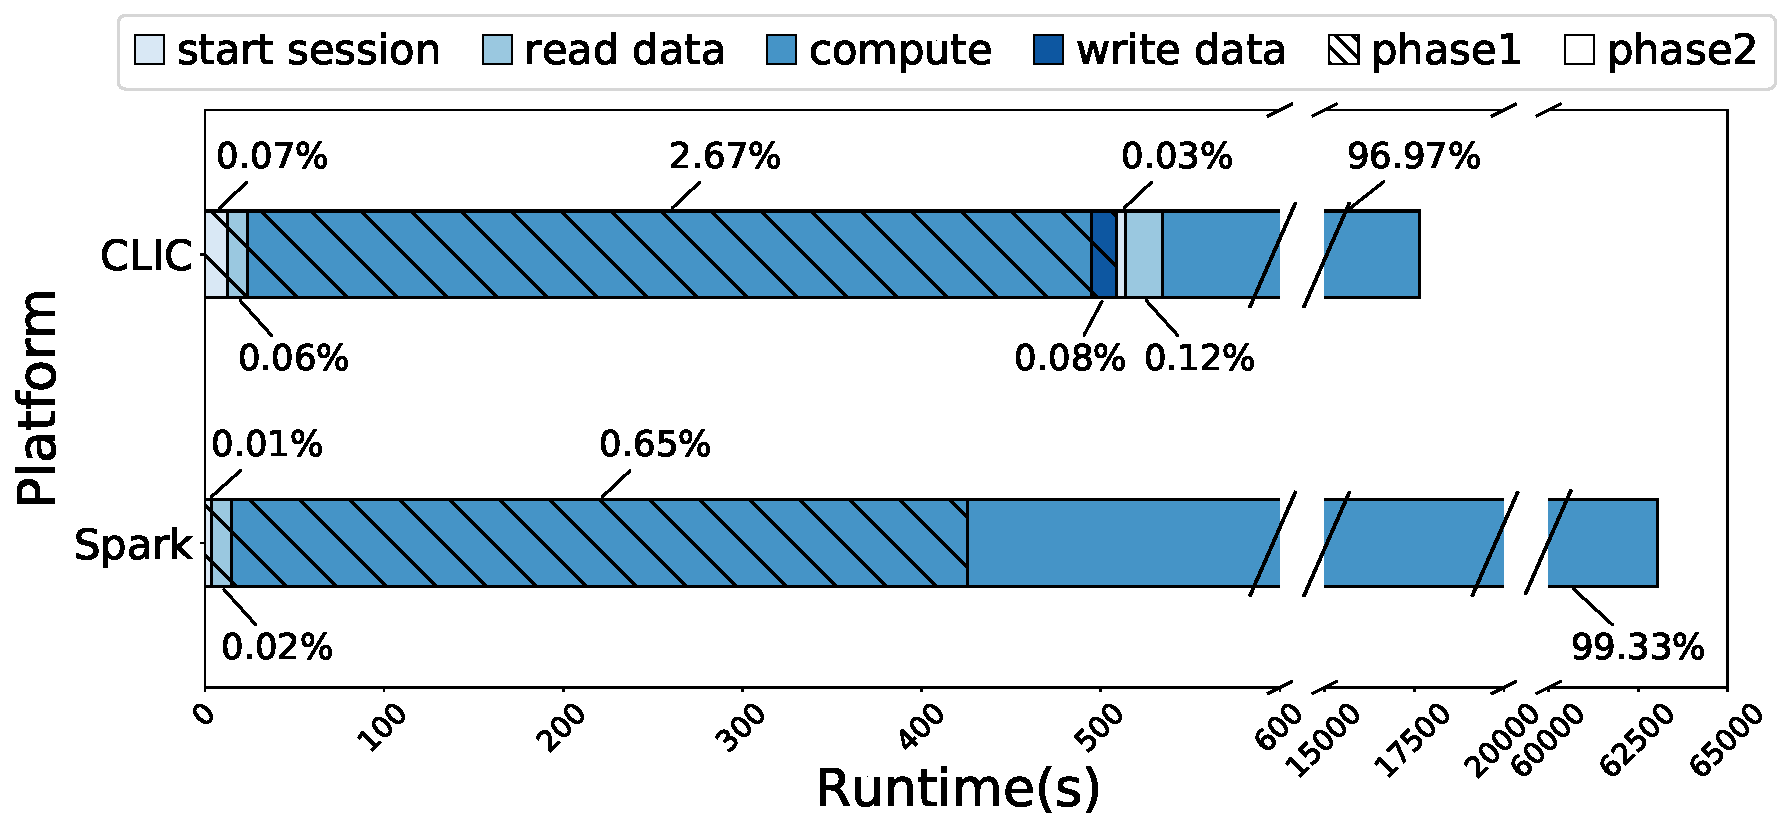
\includegraphics[width=0.8 \linewidth]{figures/chp6-nlp.pdf}
  \label{fig:hetero-nlp}
  }
  \subfigure[PageRank on Twitter Follower Network]{
  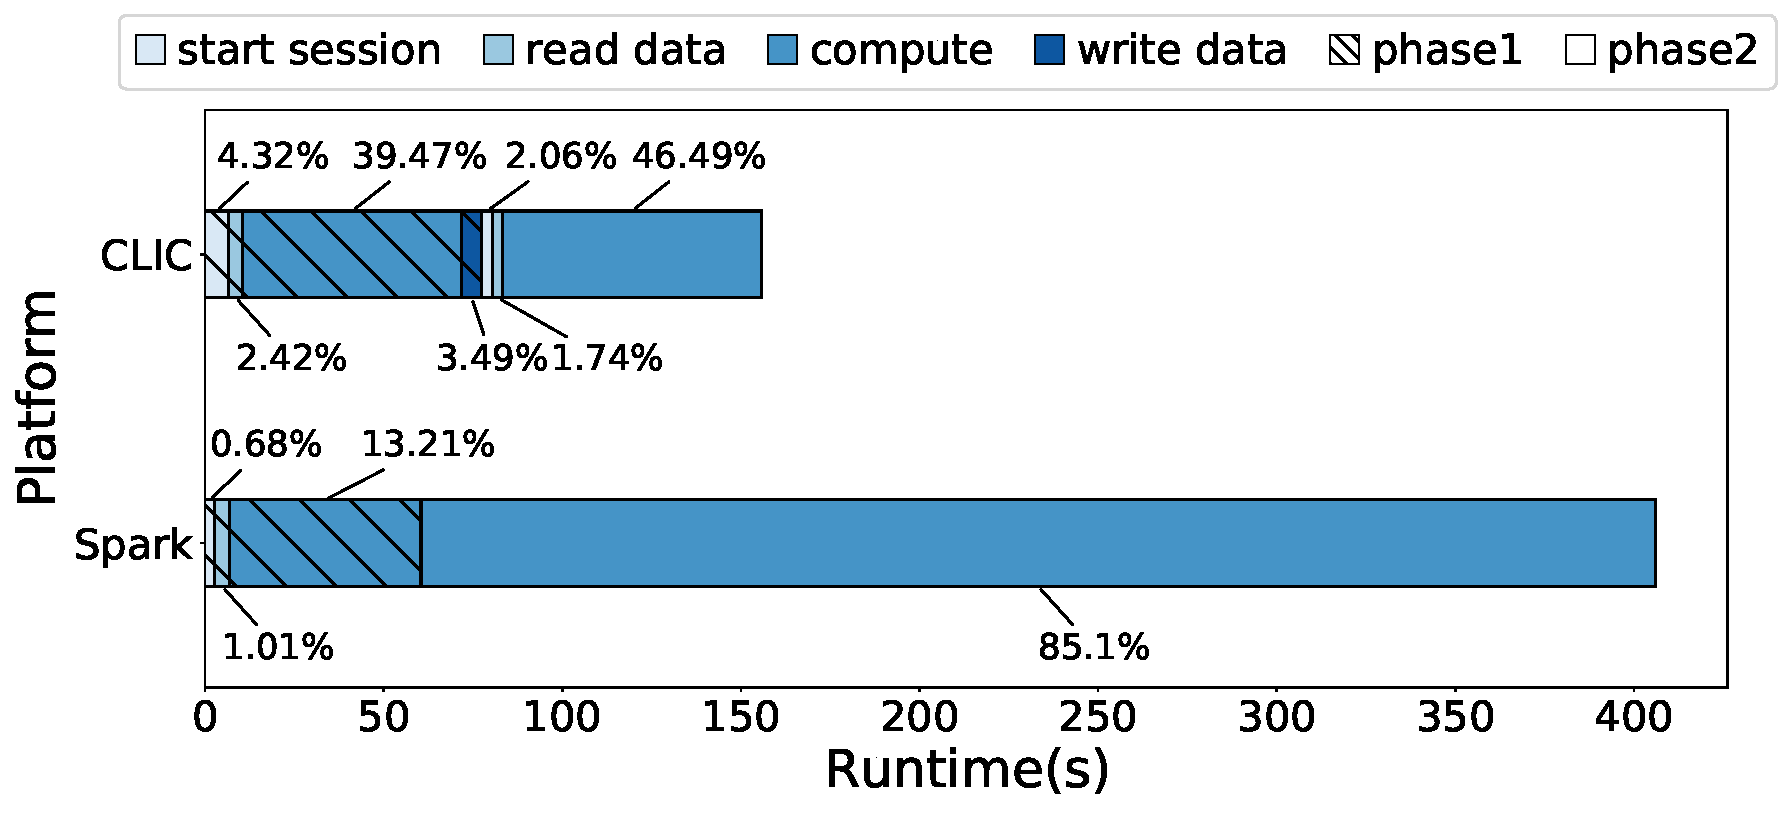
\includegraphics[width=0.8 \linewidth]{figures/chp6-pr-workflow.pdf}
  \label{fig:hetero-pr}
  }
  \caption{Performance comparison of two workflows}
  \label{fig:hetero}
\end{figure}

We consider two real-world workflows to validate CLIC’s ability to execute the workflow that contains multiple algebras. We record the time consumption of each stage when executing the workflow, including start session, data I/O, and computation.

The first workflow is the Sentiment Classification we have discussed in Section 3. It first reads and joins the two corpora using batch processing, which we call this \textit{phase1}, and then trains the deep learning model, which we call this \textit{phase2}. The training dataset is the Amazon Reviews\footnote{https://www.kaggle.com/bittlingmayer/amazonreviews} that consists of 3.4 million Amazon customer reviews (input text) and star ratings (output labels). Consider that Spark ML currently only supports a few simple machine learning models, we replace the LSTM~\cite{hochreiter1997long} with MLP (Multilayer Perception) for a fair comparison. As shown in Figure \ref{fig:hetero-nlp}, CLIC trains 3.6$\times$ faster than Spark. This is because CLIC migrates the model training process to the PyTorch platform that can use GPU for parallel training, therefore greatly reducing the training time, while the CPU-based Spark cannot obtain this benefit. Although the migration needs to read and write intermediate results across platforms, it can be seen from the percentage that its overhead is far less than the benefit from GPU acceleration. Moreover, both platforms achieve 78\% training accuracy. With the LSTM model, however, CLIC can achieve an accuracy of 97\%.

The second workflow is to perform PageRank on the Twitter follower network\footnote{https://snap.stanford.edu/data/twitter-2010.html}. It consists of extracting and filtering users who follow less than five other users (batch processing), constructing the graph, and performing PageRank (graph computing). We call the first procedure as \textit{phase1} and the last two procedures as \textit{phase2}. CLIC keeps the \textit{phase1} in Spark and migrates the phase2 to Giraph. The running time comparison between Spark and CLIC is shown in Figure \ref{fig:hetero-pr}, where the performance improvement brought by Giraph is significant comparing to the extra data movement overhead; therefore, CLIC finally demonstrates 4.8$\times$ performance improvement.

When processing data on two platforms, intermediate results need to be written from the first one and read by the following one. As shown in Figure~\ref{fig:hetero}, these overhead takes around 0.23\% and 7.29\% of the overall execution time. For the two workflows, launching tasks as containers on the cloud takes 0.07\% and 4.32\% of the execution time, respectively. Considering the performance improvements from cross-platform computing, these extra overhead is negligible. 
%We can conclude from the above two experiments that CLIC can not only execute the workflow that contains multiple algebras but also improve performance by utilizing different platforms properly.

